% !TeX program = xelatex
%%%%%%%%%%%%%%%%%%%%%%%%%%%%%%%%%%%%%%%%%%%%%%%%%%%%%%%%%%%%%%%%%%%%%%%%%%%%%%%%%%%%%%%%%%%%%%%%%%%%%%%%%%%%%%%%%%%%%%%%%%%%%%%%%%%%%%%%%%%%%%%%%%%%%%%%%%%
% Japanese manuscript generated from 論文アウトライン.md. Compile with XeLaTeX.
%%%%%%%%%%%%%%%%%%%%%%%%%%%%%%%%%%%%%%%%%%%%%%%%%%%%%%%%%%%%%%%%%%%%%%%%%%%%%%%%%%%%%%%%%%%%%%%%%%%%%%%%%%%%%%%%%%%%%%%%%%%%%%%%%%%%%%%%%%%%%%%%%%%%%%%%%%%

\documentclass[utf8]{FrontiersinHarvard}
\usepackage{url,hyperref,lineno,microtype,subcaption}
\usepackage[onehalfspacing]{setspace}
\usepackage{fontspec}
\usepackage{xeCJK}
\setmainfont{Times New Roman}
\setsansfont{Arial}
\setCJKmainfont{Yu Mincho}
\setCJKsansfont{Yu Gothic}
\setCJKmonofont{Yu Gothic}
\usepackage{tabularx,booktabs}
\usepackage{float}
\graphicspath{{figures/}}

\linenumbers

\def\keyFont{\fontsize{8}{11}\helveticabold }
\def\firstAuthorLast{Shimizu {et~al.}}
\def\Authors{Yuki Shimizu\,$^{1,*}$, Midori Ban\,$^{2}$, Hideyuki Takahashi\,$^{3}$ and Hiroshi Ishiguro\,$^{1}$}
\def\Address{$^{1}$Department of Engineering Science, Osaka University, Osaka, Japan \\
$^{2}$Kyoto Tachibana University, Kyoto, Japan \\
$^{3}$Faculty of Science and Engineering, Otemon Gakuin University, Osaka, Japan}
\def\corrAuthor{Yuki Shimizu}
\def\corrEmail{simizu.yuki@irl.sys.es.osaka-u.ac.jp}

\begin{document}
\onecolumn
\firstpage{1}

\title[接近回避葛藤を示すロボット]{内的状態としての接近回避葛藤を示すロボットの観察が観察者の個人的勇気の自己評価に及ぼす影響}

\author[\firstAuthorLast ]{\Authors}
\address{}
\correspondance{}
\extraAuth{}

\maketitle

\begin{abstract}
人前で発言する、見知らぬ相手の不適切な振る舞いに声をかける、助けを求めるといった行動は、身体的危険が大きいわけではない一方で、評価低下、拒絶、羞恥などの社会的・心理的リスクを伴う。このような場面では、何をすべきかを理解していても、恐れや困難によって価値ある行動へ向かえないことがある。本研究では、このような状況で価値ある行動へ向かう個人的勇気に注目し、ロボットが行動前の内的状態として接近回避葛藤を示すことが、観察者自身の個人的勇気の自己評価に及ぼす影響を検討した。

個人的勇気を理解するには、行動そのものだけでなく、本人が恐れや困難を抱えながら価値ある行動へ向かう内的状態も重要である。しかし、人間モデルを用いる場合、行動前の内的状態を条件間で同じ形式・強度で提示することは容易ではない。そこで本研究では、プロジェクションマッピングによる吹き出し表現を用いて、ロボットの接近動機と回避動機を観察者に提示した。研究1では、接近回避葛藤を示すロボットが勇気ある姿として知覚されるかを確認した。研究2では、研究1で確認した、勇気ある姿として知覚されるロボットの観察が、観察者自身の個人的勇気の自己評価に及ぼす影響を検討し、あわせてその効果が観察者の事前勇気傾向によって異なるかを検討した。

研究1の結果、接近回避葛藤を示したロボットは、葛藤なし条件よりも勇気ある姿として評定された。また、葛藤評定においても葛藤あり条件が高く評価され、操作の成立が確認された。研究2の結果、仮説で想定した「低群における葛藤あり・行動あり条件での高い値」は支持されなかった。一方で、観察者自身の個人的勇気の自己評価では、事前勇気傾向群と接近回避葛藤の交互作用が有意であり、低群では葛藤あり条件で高い値を示す傾向が、高群では葛藤あり条件で低い値を示す効果がみられた。行動の有無は有意な効果を示さなかった。以上より、本研究は、ロボットを媒体として個人的勇気に関わる行動前の内的状態を外在化し、その観察が観察者の個人的勇気の自己評価に対して、事前勇気傾向によって異なる意味を持つ可能性を示した。

\tiny
\keyFont{ \textbf{Keywords:} 個人的勇気、接近回避葛藤、観察学習、ヒューマンロボットインタラクション、内的状態、吹き出し表現 }
\end{abstract}

\section{イントロダクション}

日常生活には、本人にとって恐れや不安を伴う状況でも、それでも価値ある行動へ向かうことが求められる場面がある。本研究では、このような行動へ向かう力を個人的勇気として扱う。勇気は、恐怖がない状態ではなく、恐怖がある中で意味ある行動へ向かうこととして捉えられてきた \citep{rachman1984,woodard2007}。個人的勇気は、本人の文脈に照らして行動の難しさを捉えられる点で重要である。Puryらは、誰にとっても勇気ある行動として評価される一般的勇気と、その人の生活文脈や個人的制約に照らして勇気ある行動となる個人的勇気を区別した \citep{pury2007}。この観点に立つと、学習障害のある子どもが大きなテストの日に登校することや、PTSDの既往のため長年できなかったクリスマスプレゼントの包装を初めて行うことも、本人の文脈では高い恐怖と困難を伴う行為として理解される \citep{pury2007}。さらに、発言、援助要請、指摘のような行動も、本人や周囲にとって価値がありうる一方で、評価低下や拒絶といった社会的・心理的リスクを伴うため、個人的勇気の観点から検討する意義がある \citep{howard2017,vogel2007,milliken2003}。

しかし、価値ある行動だと分かっていても、人はいつも実行できるわけではない。たとえば、人前で意見を言うことは、他者からどう見られるかという不安を伴いやすい \citep{watson1969,dickerson2004}。また、困っていることを相談したり助けを求めたりすることも、他者から否定的に見られることへの懸念を伴いうる \citep{vogel2007}。職場でも、多くの従業員が問題や懸念に気づいていながら、それを上司に伝えなかった経験をもつことが報告されており、その主な理由は、否定的に見られたり、重要な関係を損なったりすることへの恐れであった \citep{milliken2003}。つまり、発言や援助要請は、本人や周囲にとって有益でありうる一方で、評価低下、関係悪化、地位低下、自己像の損失といった社会的・心理的リスクを伴う。したがって、個人的勇気を支えるには、「その行動には価値がある」と理解させるだけでは十分ではなく、リスクを感じながら、それでも行動へ向かう過程を支える必要がある。

この過程を支える方法の一つとして、本研究は観察学習に注目する。観察学習とは、他者の行動や成功する姿を見ることで、「自分にもできるかもしれない」という見込みが高まる学習である \citep{bandura1977}。観察学習は、まず外から見えやすい動作の学習で有効性が示されてきた。たとえば、水泳に恐怖をもつ子どもは、同年齢のモデルが泳ぐ姿を観察することで、技能面で良好な結果を示した \citep{weiss1998}。また、立ち座り動作の観察では、観察者の感覚運動系が反応し、動作観察そのものが運動表象を活性化しうることが報告されている \citep{chaisaen2020}。一方で、観察学習は、動作のように外から見えるものだけでなく、努力や持続性のような心理的側面にも関わりうる。SchunkとHansonは、同輩モデルの観察が子どもの自己効力感と達成行動に影響することを示した \citep{schunk1985}。また、成人が努力して目標達成を試みる姿を観察した幼児は、成人が容易に成功する姿を観察した幼児よりも、その後の困難な課題で多く試行した \citep{leonard2017}。これらの知見は、他者が困難に向き合う姿を見ることが、観察者の「自分もやってみよう」という感覚や、粘り強く取り組む姿勢を支えうることを示している。

本研究の目的は、個人的勇気を観察学習の対象として提示することで、観察者自身の個人的勇気の自己評価にどのような影響が生じるのかを明らかにすることである。個人的勇気では、「何をしたか」だけでなく、「どれほど怖かったのか」「どのようなためらいがあったのか」も重要になる \citep{pury2007}。しかし、人間モデルを用いる場合、行動前の恐れや葛藤を条件間で同じ形式・強度で提示することは容易ではない。そこで本研究では、ロボットを用いて、価値ある行動へ向かおうとする気持ちと、リスクや不利益を避けたい気持ちが同時に存在する状態を接近回避葛藤として表現させ、その観察が観察者自身の個人的勇気の自己評価に及ぼす影響を検討する。

本研究では二つの研究を実施する。研究1では、どのようなロボット表現が「勇気を感じられる行動」として知覚されるのかを明らかにする。具体的には、接近回避葛藤を示すロボットが、葛藤を示さないロボットよりも勇気ある姿として知覚されるかを確認し、研究2で用いる刺激の妥当性を検討する。研究2では、研究1で確認した、勇気ある姿として知覚されるロボットを観察させ、その観察が観察者自身の個人的勇気の自己評価に影響するかを明らかにする。さらに、接近回避葛藤の提示による効果と、価値ある行動へ向かう行動選択の観察効果を切り分けるため、葛藤の有無と行動の有無を分けて操作する。これにより、本研究は、個人的勇気を観察学習の対象として扱う際に、行動そのものだけでなく、行動前の内的状態を提示することがどのような意味をもつのかについて知見を提供する。また、ロボットを用いて外から見えにくい内的状態を可視化し、勇気を支える観察学習に利用するための方法的示唆を提供する。

\section{関連研究}

\subsection{個人的勇気と行動前の内的状態}

勇気研究では、勇気は恐怖の不在ではなく、恐怖を抱えながらも行動へ向かうこととして扱われてきた。Rachmanは、恐怖の強い人であっても勇気ある行為を行いうることを論じている \citep{rachman1984}。NortonとWeissは、恐怖喚起場面における行動接近と勇気の関係を検討した \citep{norton2009}。WoodardとPuryも、勇気を、脅威や恐怖がある状況で意味ある目的のために行動する構成概念として整理している \citep{woodard2007}。これらの研究は、勇気を単なる危険選好や恐怖の低さではなく、恐怖がある状況での接近行動として捉える基盤を与えている。

その中でもPuryらは、誰にとっても勇気ある行動として評価される一般的勇気と、その人の生活文脈や個人的制約に照らして勇気ある行動となる個人的勇気を区別した \citep{pury2007}。個人的勇気の高い行動は、恐怖、困難、個人的制約を伴う行為として特徴づけられる。この区別からみると、同じ行動であっても、それが勇気あるものかどうかは、行為者がどのような恐れや困難を抱えていたかによって変わりうる。したがって、個人的勇気を扱うには、外から見える行動だけでなく、その行動に先立つ内的状態を考慮する必要がある。

近年、勇気が生じるメカニズムを説明するモデルでも、この行動前の内的状態に注目している。Chowkaseらは、勇気を、状況の認知、価値や意味の評価、行為可能性の評価、行動決定が連鎖する過程として説明している \citep{chowkase2024}。この過程では、価値ある行動へ向かう理由と、行動に伴うリスクや不利益を避けようとする理由が同時に存在しうる。これは、接近動機と回避動機が同時に働く接近回避葛藤として理解できる \citep{lewin1931,miller1944}。ただし、これらの研究は、勇気の定義や過程を明らかにするものであり、他者の内的状態を観察させることで観察者自身の個人的勇気の自己評価が変化するかは直接検討していない。

\subsection{観察学習とモデルの事前特性依存性}

観察学習研究では、他者の行動やその結果を観察することで、観察者の行動、動機づけ、自己効力感が変化しうることが示されてきた。Banduraは、自己効力感を形成する情報源の一つとして代理経験を位置づけ、他者が課題に成功する姿を観察することが「自分にもできる」という見込みに影響しうると論じた \citep{bandura1977}。SchunkとHansonは、同輩モデルの観察が子どもの自己効力感と達成行動に影響することを示した \citep{schunk1985}。これらの研究は、他者が行動する姿を見ることが、観察者自身もその行動を実行できるという認知に影響を及ぼす可能性を示している。

モデルの効果は、モデルがどのような状態で行動するかによっても変わる。Schunkらは、最初から容易に成功する熟達モデルと、困難を示しながら徐々に対処していく対処モデルを比較し、対処モデルの観察が自己効力感や課題遂行を高めることを示した \citep{schunk1987}。SchunkとHansonも、困難や否定的感情を示しながら対処するモデルが学習自己効力感に影響することを示している \citep{schunk1989}。Leonardらは、成人が努力して目標達成を試みる姿を観察した幼児が、成人が容易に成功する姿を観察した幼児よりも、その後の困難な課題で多く試行することを示した \citep{leonard2017}。これらの知見は、困難や努力を含む過程の観察が、観察者の自己効力感や持続性を支えうることを示している。

一方で、同じモデルであっても、観察者の事前特性によって受け取られ方は異なりうる。Braaksmaらは、観察学習においてモデルと観察者の類似性や熟達度が重要であることを示している \citep{braaksma2002}。Lucasらは、課題が難しい場合には人は他者の判断や行動を手がかりにしやすいが、自己効力感が高い人はそのような他者からの影響を受けにくいことを示した \citep{lucas2006}。これらの知見から、観察学習を用いる場合には、モデルの特徴だけでなく、観察者がそのモデルをどのように受け取るかに関わる事前特性も考慮する必要がある。したがって、本研究でも、ロボットによる葛藤提示の効果を検討する際に、観察者の事前特性を考慮する。

\subsection{ロボット・人工エージェントによるモデリング}

観察学習のモデルは人間に限られない。人工エージェントやアバターを用いた研究では、視覚的に存在するエージェントや自己に似たアバターが、観察者の態度、自己効力感、後続行動に影響しうることが示されている \citep{rosenberg2008,fox2009}。また、社会的ロボットに関する研究でも、人はロボットを社会的モデルとして扱い、その行動や社会的役割を手がかりにモデリングを行いうることが示されている \citep{xu2023}。さらに、ロボットの励まし方が参加者自身の後続の励まし方へ影響することも報告されている \citep{higashino2023}。

これらの研究は、ロボットや人工エージェントが、観察者に影響する社会的モデルとして機能しうることを示している。ただし、本稿で取り上げた研究は、態度、自己効力感、運動、励まし方などを対象としており、個人的勇気そのものを扱ったものではない。また、本稿で確認した範囲では、モデルが行動前にどのような恐れや葛藤を抱えているかを明示し、その観察が観察者自身の個人的勇気の自己評価に及ぼす影響を検討した研究は限られている。したがって、ロボットを用いて個人的勇気に関わる内的状態を観察可能な形で提示することには、既存のモデリング研究を拡張する意義がある。

\subsection{ロボットによる内的状態の外在化}

本研究でロボットを用いる実験上の理由は、行動や発話に加えて、視覚表現を条件間で統制しやすい点にある。人間モデルでも、表情、声、沈黙、自己開示などから内的状態を推測することはできる。しかし、本研究のように、恐れ、ためらい、接近動機、回避動機の有無を、同じシナリオ内で条件間にそろえて提示するには、人工的な媒体を用いる方が適している。そこで本研究では、ロボットの動作や発話に加えて吹き出し表現を用い、内的状態を外在化した刺激として提示した。

吹き出し表現に関して、Nitadaらは、ビデオ会議場面においてロボットの頭部付近に吹き出しを表示し、その中にユーザーの顔を描く方法を提案した \citep{nitada2021}。その結果、吹き出しあり条件では、ロボットが自分を見ているという感覚が高まった。同研究は、吹き出しがロボットの注意や心的焦点を視覚的に表す手段として機能しうることを示している。ただし、この研究で扱われたのは注意の向きであり、勇気に関わる接近動機と回避動機の葛藤ではない。

以上を踏まえると、先行研究は、個人的勇気が恐怖や困難を伴う行動であること、観察学習が自己効力感や行動可能性に影響しうること、ロボットや人工エージェントが社会的モデルとして機能しうることを示してきた。しかし、本稿で確認した範囲では、個人的勇気に関わる行動前の内的状態、特に接近動機と回避動機の葛藤をロボットによって外在化し、その観察が観察者自身の個人的勇気の自己評価に及ぼす影響を検討した研究は十分ではない。本研究は、この未検討の点に着目し、接近回避葛藤を示すロボットの観察が観察者自身の個人的勇気の自己評価にどのように関わるのかを検討する。

\section{動画刺激の設計}

\subsection{刺激場面}

本研究では、ロボットが公園でごみをポイ捨てしている人物を見かける場面を動画刺激として用いた。公園でのポイ捨ては、公共空間における共有規範への違反として理解されやすい。実際に、ポイ捨ては記述的規範と命令的規範の影響を検討する代表的な課題として用いられてきた \citep{cialdini1990}。また、公共空間での観察研究では、既存のごみの存在がポイ捨てを増やし、ゴミ箱の利用可能性がポイ捨てを減らすことが示されており、ポイ捨ては日常的に生じる規範違反でありながら、環境や規範手がかりに左右される行動として位置づけられる \citep{schultz2013}。さらに、ごみや落書きのような無秩序の手がかりは、他の規範違反を誘発しうることも示されている \citep{keizer2008}。そのため、この場面で相手に注意することには、公園をきれいに保つ、相手がポイ捨てをやめるきっかけを作る、ポイ捨てが許容されないという規範を確認するといった価値がある。一方で、見知らぬ相手に注意することには、相手に怒られる、無視される、否定的に見られるといった社会的・心理的リスクも伴う。公園でのポイ捨ては、社会的統制行動を検討する先行研究でも刺激場面として用いられており、見知らぬ他者の規範違反に対する介入を扱う場面として一定の妥当性をもつ \citep{chekroun2002}。さらに、フィールド研究では、見知らぬ他者の規範違反に対する制裁には直接的な注意だけでなく間接的な方法もあり、直接的な注意には相手からの反発可能性を含むコストが伴いうることが示されている \citep{balafoutas2014}。社会的勇気の研究では、対人的リスクを伴いながら価値ある行動に向かうことが重要な特徴として整理されている \citep{howard2017}。したがって、公園でのポイ捨てを注意する場面は、身体的危険が極端に高い場面ではない一方で、価値ある行動と対人的リスクが同時に存在し、本人にとってためらいや葛藤が生じうるため、個人的勇気を検討する刺激場面として適している。

\begin{figure}[htbp]
\centering
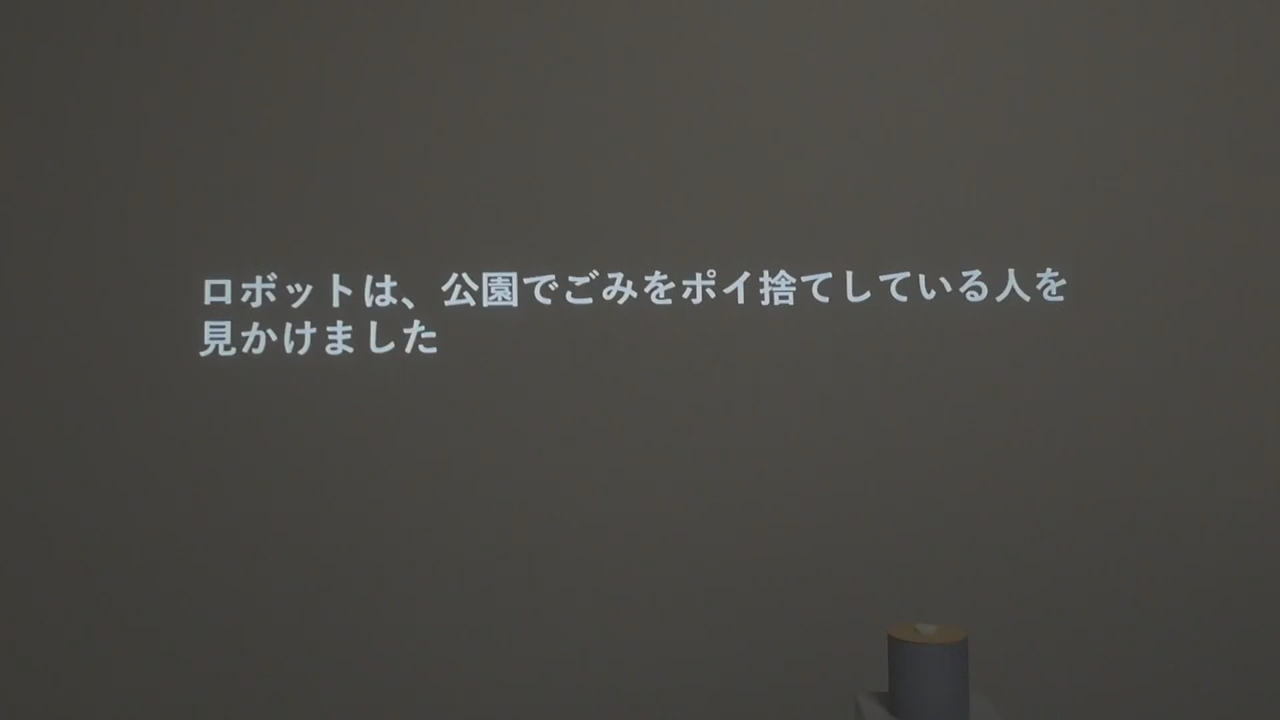
\includegraphics[width=0.86\linewidth]{figures/fig1_scene.png}
\caption{動画刺激における状況説明}
\label{fig:scene}
\end{figure}


\subsection{動画刺激の共通構成}

動画刺激では、公園場面そのものを実写映像として提示するのではなく、状況説明文と吹き出し表現によって場面を構成した。動画の冒頭では、「ロボットは、公園でごみをポイ捨てしている人を見かけました」という状況説明を提示した。その後、吹き出し内に「あ、ごみをポイ捨てしている人がいる」という状況認知を提示し、続いて注意すべき状況であることを示す認知を提示した。吹き出しはロボットの頭部付近に提示され、ロボットの発話ではなく、行動前の内的状態を表す視覚的表現として用いた。動画はいずれも1280×720ピクセルで作成され、研究1の動画は約50〜54秒、研究2の動画は約49〜50秒であった。

\subsection{接近動機と回避動機}

本研究では、価値ある行動へ向かおうとする理由を接近動機、行動に伴うリスクや不利益を避けたい理由を回避動機として設定した。接近動機は、「注意したら公園がきれいになるかもしれない」「注意したらあの人がポイ捨てをやめるきっかけになるかも」という内容であった。これらは、注意行動によって望ましい結果が生じる可能性を示すものである。回避動機は、「注意して怒鳴られたら嫌だな」「注意しても無視されて相手にされないかも」という内容であった。これらは、注意行動によって生じうる社会的・心理的リスクを示すものである。本研究では、これらの接近動機と回避動機の組み合わせによって、価値ある行動へ向かう理由と、その行動を避けたい理由が同時に存在する状態を表現した。これは、接近動機と回避動機が同時に働く接近回避葛藤として位置づけられる \citep{lewin1931,miller1944}。

\begin{figure}[htbp]
\centering
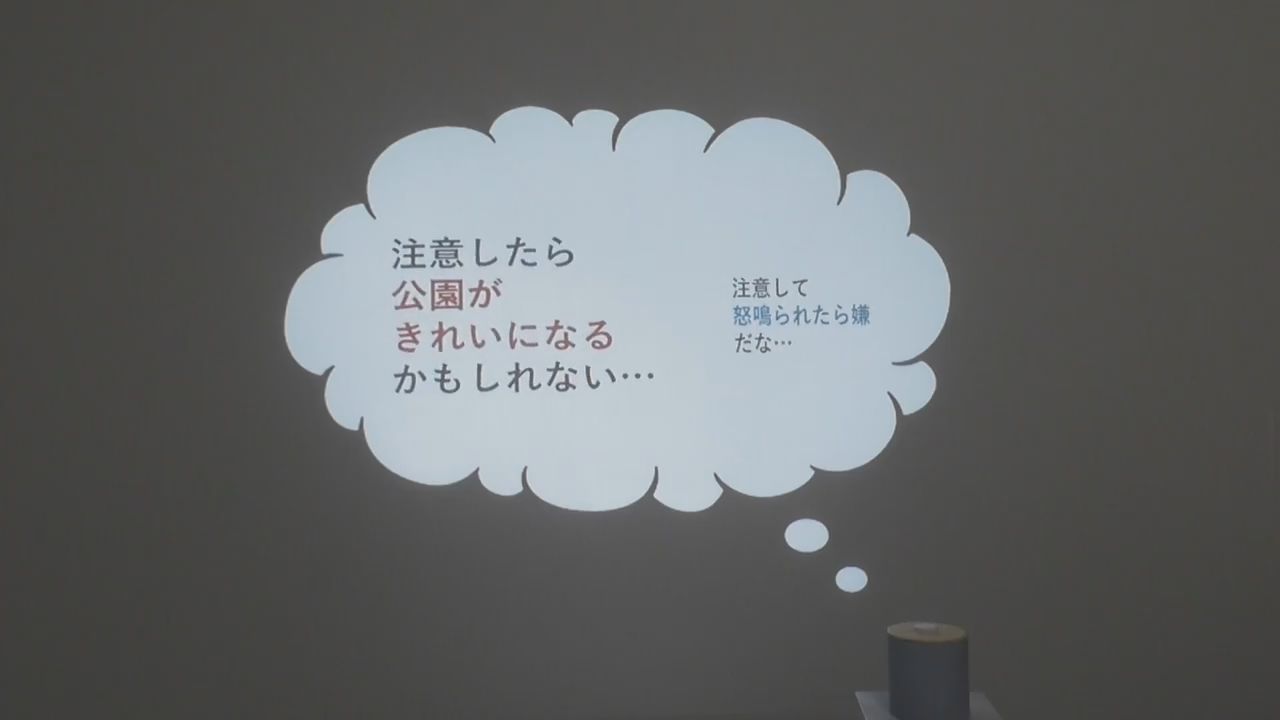
\includegraphics[width=0.86\linewidth]{figures/fig2_conflict.png}
\caption{接近動機と回避動機を同時に提示した例}
\label{fig:approach_avoidance}
\end{figure}


以上の共通設計により、本研究では、行動前の内的状態を、観察者が視覚的に把握できる形で提示した。各研究における条件操作の詳細は、それぞれの方法節で述べる。

\section{研究1：接近回避葛藤を示すロボットは勇気ある姿として知覚されるか}

\subsection{目的}

研究1の目的は、研究2で用いる提示が、勇気ある姿として知覚されるかを確認することであった。具体的には、内的状態として接近回避葛藤を示すロボットが、葛藤なし条件よりも勇気ある姿として知覚されるかを検討した。あわせて、提示した内的状態が接近回避葛藤として知覚されるかを葛藤評定で確認し、研究2で用いる提示方法を探索的に選定した。

接近回避葛藤は、接近動機と回避動機が同時に働く状態として説明される \citep{lewin1931,miller1944}。一方で、葛藤の経験は、時間的な揺れとしても生じうる。そのため研究1では、接近動機と回避動機を順番に示す逐次提示と、両者を同時に示す同時提示の二つを候補とした。研究1では、勇気評定を優先し、差がない場合には葛藤評定を参照して研究2の提示方法を選定することとした。

\subsection{方法}

\subsubsection{Conditions}

研究1は、葛藤の有無と提示方法を要因とする参加者内計画であった。葛藤の有無には、葛藤なし条件と葛藤あり条件を設定した。提示方法には、逐次提示と同時提示を設定した。研究1では、最終的な行動の有無による影響を混入させないため、全条件でロボットが注意する行動を提示した。

刺激動画では、ロボットは公園でごみをポイ捨てしている人を見かけた後、吹き出しによって状況認知と動機を示した。葛藤あり条件では接近動機と回避動機を提示し、葛藤なし条件では接近動機のみを提示した。同時提示条件では、接近動機と回避動機を同時に提示し、交互に拡大縮小させた。逐次提示条件では、二つの動機を順番に提示した。最後に、全条件でロボットが「すみません、そこはごみを捨てる場所じゃありませんよ」と発話した。

\begin{table}[htbp]
\centering
\small
\caption{研究1の条件}
\begin{tabularx}{\linewidth}{lXlX}
\toprule
研究1の条件 & 内的状態の内容 & 提示方法 & 最後の注意発話 \\
\midrule
葛藤なし・逐次提示 & 接近動機のみ & 接近動機を順番に提示 & あり \\
葛藤なし・同時提示 & 接近動機のみ & 複数の接近動機を同時に提示し、交互に強調 & あり \\
葛藤あり・逐次提示 & 接近動機と回避動機 & 接近動機と回避動機を順番に提示 & あり \\
葛藤あり・同時提示 & 接近動機と回避動機 & 接近動機と回避動機を同時に提示し、交互に強調 & あり \\
\bottomrule
\end{tabularx}
\end{table}


\subsubsection{Measurement}

従属変数は、ロボットの勇気評定と葛藤評定であった。いずれの評定も、各動画を観察した後に1〜7の7件法で回答を求め、項目平均を得点として用いた。勇気評定は、日本語版勇気尺度（CM-J）の6項目をロボット評定用に変更して作成した \citep{geshi2023}。CM-Jは、恐怖や不安を感じながらも行動へ向かう傾向を測定する尺度であり、信頼性と妥当性が確認されている \citep{geshi2023}。研究1では、観察者自身の勇気ではなく、ロボットがどの程度勇気ある姿として見えたかを測定するため、各項目の主語を「このロボットは」に変更し、語尾を「〜ように見えた」「〜していた」といった観察評定の表現に変更した。分析では、以下の6項目の平均値を勇気評定得点とした。

\begin{table}[htbp]
\centering
\small
\caption{勇気評定項目}
\begin{tabularx}{\linewidth}{cX}
\toprule
項目 & 勇気評定項目 \\
\midrule
1 & このロボットは、自身の恐怖に立ち向かうように見えた。 \\
2 & このロボットは、たとえ強い恐れを感じていても、やるべきことをやるまでは逃げ出さないように見えた。 \\
3 & このロボットは、たとえ危険に思えることがあっても、それをやっていた。 \\
4 & このロボットは、何か心配や不安があっても、とにかく行動を起こすか、立ち向かっていた。 \\
5 & このロボットは、恐ろしいことであっても、立ち向かうべき重大な理由があれば、立ち向かっていた。 \\
6 & このロボットは、たとえ自身を脅かすものがあっても、引き下がらないように見えた。 \\
\bottomrule
\end{tabularx}
\end{table}


葛藤評定は、ロボットが接近動機と回避動機のあいだで迷っているように見える程度を測定するため、自作項目を用いた。項目作成では、接近回避葛藤の定義 \citep{lewin1931,miller1944} を踏まえ、目の前のことをしたいが怖くてためらうこと、行動に迷いや揺れがあること、やりたい気持ちとやりたくない気持ちが混在していること、自分の行動を決めかねていることを、接近回避葛藤の観察可能な側面として文章化した。分析では、以下の4項目の平均値を葛藤評定得点とした。また、この4項目による葛藤評定が直接的な葛藤判断と対応するかを確認するため、「このロボットは、葛藤しているように見えた。」という直接項目も取得した。

\begin{table}[htbp]
\centering
\small
\caption{葛藤評定項目}
\begin{tabularx}{\linewidth}{cX}
\toprule
項目 & 葛藤評定項目 \\
\midrule
1 & このロボットは、目の前のことをやりたいけれど、怖くてためらっているように見えた。 \\
2 & このロボットは、自分の行動に迷いや揺れがあるように見えた。 \\
3 & このロボットは、やりたいという気持ちとやりたくない気持ちが混在しているように見えた。 \\
4 & このロボットは、自分の行動を決めかねているように見えた。 \\
\bottomrule
\end{tabularx}
\end{table}


\subsubsection{Procedure}

研究1は、Yahoo!クラウドソーシング上で実施した。参加者は4条件の動画を視聴し、各動画の視聴後にロボットの勇気評定と葛藤評定に回答した。動画の提示順は、参加者ごとにランダム化した。回答データには、動画内容の理解確認項目および注意確認項目を含めた。

\subsubsection{Participants}

動画内容の理解確認項目および注意確認項目に基づいて除外を行い、最終的に131名を分析対象とした。分析対象者の年齢は18〜29歳であり、平均年齢は24.26歳であった（SD = 3.36）。性別は、女性76名、男性52名、分からない・答えたくない3名であった。

研究1では、葛藤あり条件は葛藤なし条件よりもロボットの勇気評定が高いと予測した。また、操作チェックとして、葛藤あり条件は葛藤なし条件よりも葛藤評定が高いと予測した。提示方法については、逐次提示と同時提示のどちらが勇気ある姿として知覚されるかを探索的に比較した。

\subsection{結果}

まず、勇気評定と葛藤評定がそれぞれ一つの尺度得点として扱えるかを確認した。因子分析で得られる因子の符号は任意であるため、因子負荷量は絶対値で報告する。勇気評定6項目のCronbachのα係数は .925 であった。1因子解を指定した因子分析では、第1因子の因子負荷量は .727〜.855 であり、寄与率は68.0\%であった。また、第1固有値は4.396であり、第2固有値以下はいずれも1を下回った。したがって、6項目の平均値を勇気評定得点として用いた。葛藤評定4項目のCronbachのα係数は .928 であった。1因子解を指定した因子分析では、第1因子の因子負荷量は .845〜.898 であり、寄与率は76.5\%であった。また、第1固有値は3.293であり、第2固有値以下はいずれも1を下回った。さらに、4項目から算出した因子得点と直接項目との相関を確認したところ、高い正の相関がみられた（r = .887, p \textless{} .001）。したがって、4項目の平均値を葛藤評定得点として用いた。

勇気評定では、葛藤あり条件の方が葛藤なし条件よりも高かった。葛藤の主効果は有意であった（F(1, 130) = 12.216, p = .000649, 一般化η² = .020）。一方、提示方法の主効果は有意ではなく（F(1, 130) = 2.657, p = .106）、交互作用も有意ではなかった（F(1, 130) = 0.906, p = .343）。

\begin{figure}[htbp]
\centering
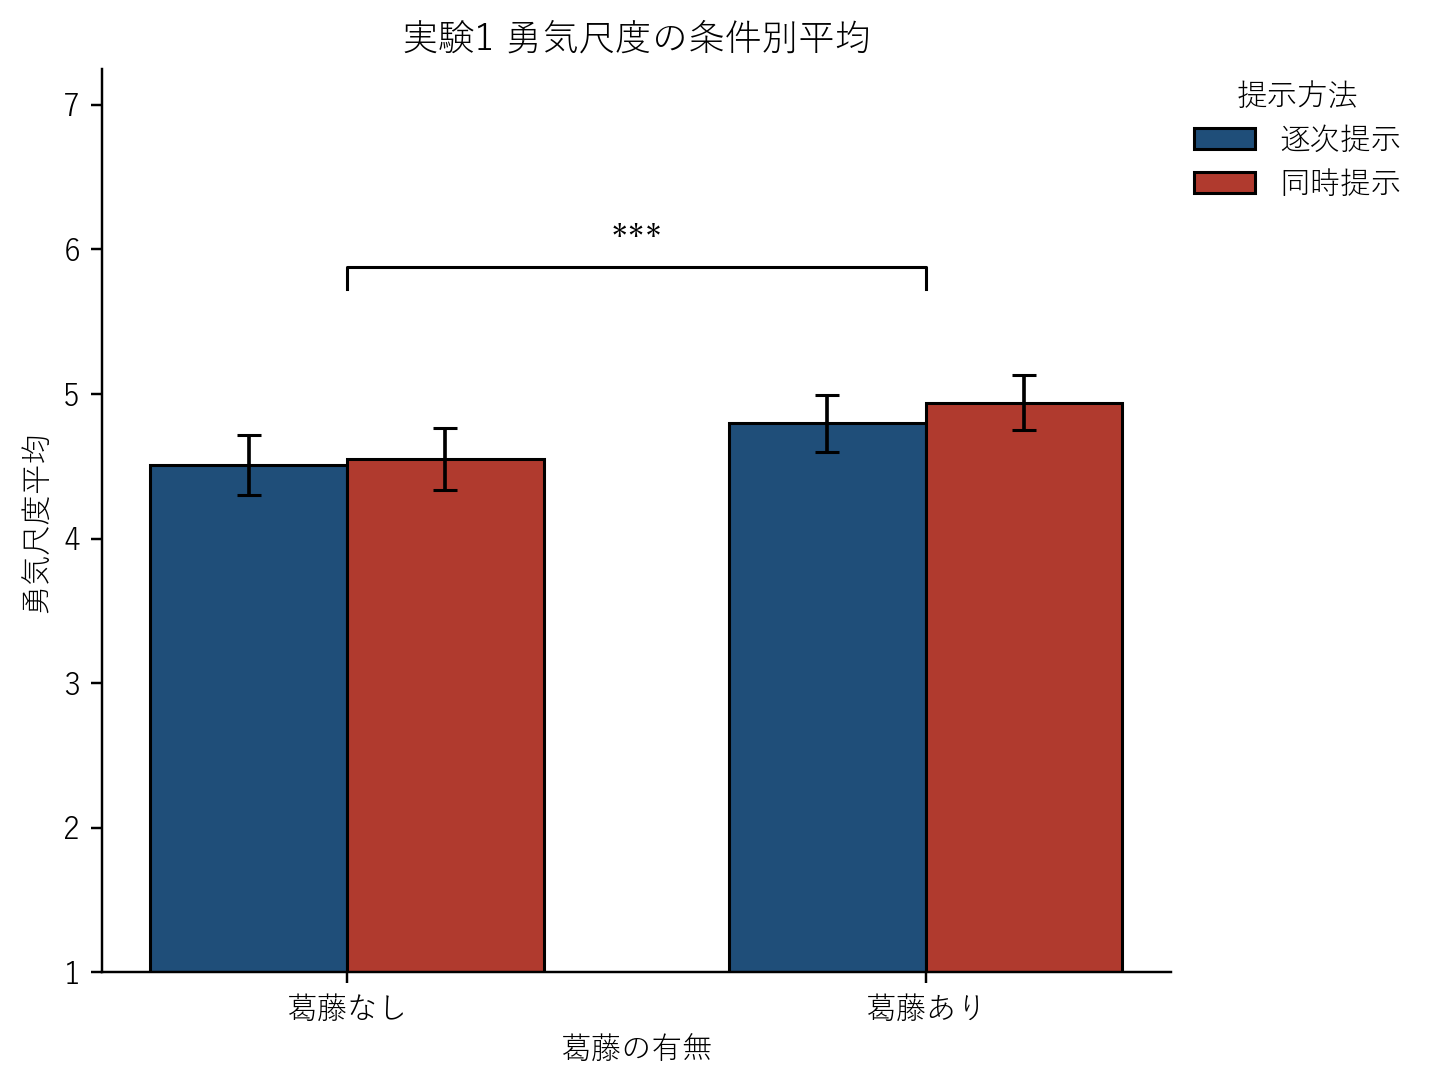
\includegraphics[width=0.86\linewidth]{figures/fig3_study1_courage.png}
\caption{研究1 勇気評定の条件別平均}
\label{fig:study1_courage}
\end{figure}


葛藤評定では、葛藤あり条件の方が葛藤なし条件よりも高く、同時提示の方が逐次提示よりも高かった。葛藤の主効果は有意であった（F(1, 130) = 79.558, p \textless{} .001, 一般化η² = .170）。また、提示方法の主効果も有意であり（F(1, 130) = 46.448, p \textless{} .001, 一般化η² = .039）、交互作用も有意であった（F(1, 130) = 4.924, p = .028）。

\begin{figure}[htbp]
\centering

\includegraphics[width=0.86\linewidth]{figures/fig4_study1_conflict.png}
\caption{研究1 葛藤評定の条件別平均}
\label{fig:study1_conflict}
\end{figure}


\subsection{考察}

研究1では、接近回避葛藤を示したロボットが、葛藤なし条件よりも勇気ある姿として評定された。これは、行動そのものを同じにしても、行動前に接近動機と回避動機の葛藤を示すことで、その行動が本人にとって恐れや困難を伴うものとして理解されやすくなることを示している。この解釈は、個人的勇気の高い行動が恐怖や困難を伴うとする整理とも整合する \citep{pury2007}。したがって、個人的勇気に関わる行動前の内的状態を外在化することは、ロボットの行動を勇気ある姿として観察者に提示するうえで有効であると考えられる。

また、葛藤評定では、葛藤あり条件が葛藤なし条件より高く評定された。これは、吹き出しによる接近動機と回避動機の提示が、観察者に接近回避葛藤として知覚されたことを示している。提示方法については、勇気評定では逐次提示と同時提示の差はみられなかった。一方で、葛藤評定では同時提示の方が高かった。したがって、同時提示は「より勇気を感じさせる提示方法」ではなく、「葛藤をより明瞭に伝える提示方法」として研究2に採用することが妥当であると判断した。

研究1では、接近回避葛藤を示すロボットが勇気ある姿として知覚されることを確認し、研究2で用いる提示の妥当性を支える知見を得た。これを踏まえ、研究2では、研究1で選定した同時提示を用い、本研究の主目的である、勇気ある姿として知覚されるロボットの観察が観察者自身の個人的勇気の自己評価に及ぼす影響を検討した。

\section{研究2：勇気ある姿として知覚されるロボットの観察は観察者自身の個人的勇気の自己評価に影響するか}

\subsection{目的}

研究2の目的は、研究1において勇気ある姿として知覚されることが確認されたロボットを観察することが、観察者自身の個人的勇気の自己評価にどう影響するかを検討することであった。あわせて、その影響が事前勇気傾向によって異なるかを検討した。

研究2では、葛藤の有無と行動の有無を分けて操作した。これは、勇気が恐れや困難を伴う状況で価値ある行動へ向かうこととして整理されているためである \citep{rachman1984,woodard2007,norton2009}。また、Chowkaseらのモデルでも、勇気は状況認知、価値評価、行為可能性の評価、行動決定が連鎖する過程として説明されている \citep{chowkase2024}。接近回避葛藤のみを示す条件では、行動前の内的状態の観察効果が示される一方で、行動のみを示す条件では、価値ある行動へ向かう行動選択の観察効果にとどまる可能性がある。そこで、葛藤の有無と行動の有無を分けて操作し、接近回避葛藤のみ、行動のみ、両方がそろった場合の違いを切り分けた。

研究2では、接近回避葛藤と行動の有無が観察者自身の個人的勇気の自己評価に及ぼす影響は、事前勇気傾向によって異なると予測した。特に、事前勇気傾向が低い群では、葛藤あり・行動あり条件で観察後の個人的勇気自己評価得点が高い値を示すと予測した。根拠として、勇気の自己評価が低い低群は、葛藤場面において行動を起こすことに困難を感じている群である。先行研究では、困難を示しながら徐々に対処するモデルの観察が、自己効力感や課題遂行を高めうることが示されている \citep{schunk1987,schunk1989}。また、課題が難しい場合には人は他者の判断や行動を手がかりにしやすいが、自己効力感が高い者は他者影響から相対的に独立しやすいことも示されている \citep{lucas2006}。葛藤あり・行動あり条件は、回避動機と接近動機の併存を示しつつ、行動へ向かう選択を提示する。すなわち、低群が直面する困難に寄り添いながらそれを乗り越える過程を提示できるため、低群において観察後の個人的勇気自己評価得点が最も高い値を示すと予測した。

\subsection{方法}

\subsubsection{Conditions}

研究2では、事前勇気傾向群を参加者間要因、葛藤の有無と行動の有無を参加者内要因とする3要因混合計画を用いた。事前勇気傾向群は、刺激提示前のCM-J得点に基づいて低群と高群に分類した。葛藤の有無は、接近動機と回避動機を同時に示すか、一方の動機のみを示すかによって操作した。行動の有無は、ロボットが注意の発話を行うかどうかによって操作した。

刺激動画では、研究1と同様に、ロボットが公園でごみをポイ捨てしている人を見かける場面を提示した。ロボットは状況認知を示した後、条件に応じて接近動機と回避動機を吹き出しで提示した。葛藤あり条件では、接近動機と回避動機を同時に提示し、交互に拡大縮小させた。葛藤なし・行動あり条件では、接近動機のみを提示した。葛藤なし・行動なし条件では、回避動機のみを提示した。

行動あり条件では、動機提示後にロボットが「すみません、そこはごみを捨てる場所じゃありませんよ」と発話した。行動なし条件では、動機提示後にロボットは発話せず、注意行動を行わない状態を提示した。

\begin{table}[htbp]
\centering
\small
\caption{研究2の条件}
\begin{tabularx}{\linewidth}{lXlX}
\toprule
研究2の条件 & 内的状態の内容 & 提示方法 & 最後の注意発話 \\
\midrule
葛藤なし・行動なし & 回避動機のみ & 回避動機を提示し、強調 & なし \\
葛藤なし・行動あり & 接近動機のみ & 接近動機を提示し、強調 & あり \\
葛藤あり・行動なし & 接近動機と回避動機 & 同時提示し、交互に強調 & なし \\
葛藤あり・行動あり & 接近動機と回避動機 & 同時提示し、交互に強調 & あり \\
\bottomrule
\end{tabularx}
\end{table}


\subsubsection{Measurement}

研究2では、刺激提示前の個人的勇気傾向、刺激提示後における観察者自身の個人的勇気の自己評価、およびロボットの葛藤評定を測定した。いずれの評定も、1〜7の7件法で回答を求めた。個人的勇気は、日本語版勇気尺度（CM-J）の6項目を用いて測定した \citep{geshi2023}。CM-Jは本来、恐怖や不安を感じながらも行動へ向かう傾向の個人差を測定する尺度である \citep{geshi2023}。研究2では、刺激提示前のCM-J得点を観察者の事前勇気傾向を表す指標として用いた。一方、刺激提示後のCM-J得点は、長期的な勇気特性そのものの変化ではなく、刺激提示直後における観察者自身の個人的勇気の自己評価として扱った。分析では、6項目の平均値を個人的勇気自己評価得点とした。

葛藤評定は、研究1と同じ4項目を用いた。分析では、4項目の平均値を葛藤評定得点とした。また、この4項目による葛藤評定が直接的な葛藤判断と対応するかを確認するため、研究1と同様に「このロボットは、葛藤しているように見えた。」という直接項目も取得した。

\subsubsection{Procedure}

研究2は、Yahoo!クラウドソーシング上で実施した。参加者は、刺激提示前にCM-Jに回答した。その後、4条件の動画を視聴し、各動画の視聴後に観察者自身の個人的勇気の自己評価とロボットの葛藤評定に回答した。動画の提示順は固定順であった。回答データには、動画内容の理解確認項目および注意確認項目を含めた。

\subsubsection{Participants}

研究1と同様に、動画内容の理解確認項目および注意確認項目に基づいて除外を行い、最終的に126名を分析対象とした。分析対象者の年齢は18〜29歳であり、平均年齢は24.11歳であった（SD = 3.62）。性別は、男性55名、女性71名であった。事前CM-J得点に基づき、得点が4未満の参加者を低群、4以上の参加者を高群に分類した。低群は69名、高群は57名であった。

\subsection{結果}

観察者自身の個人的勇気の自己評価では、仮説で想定した、低群における葛藤あり・行動あり条件での高い値は支持されなかった。一方で、事前勇気傾向群と接近回避葛藤の交互作用が有意であった（F(1, 124) = 7.513, p = .007, 偏η² = .057）。

単純主効果では、事前勇気傾向が低い群において、葛藤あり条件で観察後の個人的勇気自己評価得点が高い値を示す傾向がみられた（葛藤あり M = 3.104, 葛藤なし M = 2.982, t = 1.980, p = .052, d = .238）。一方、事前勇気傾向が高い群では、葛藤あり条件で観察後の個人的勇気自己評価得点が有意に低かった（葛藤あり M = 4.757, 葛藤なし M = 4.858, W = 404.0, p = .038, d = -.271）。

行動の有無は、観察後の個人的勇気自己評価得点に有意な効果を示さなかった。したがって、ロボットが実際に注意行動を行ったかどうかは、観察者自身の個人的勇気の自己評価に対して明確な追加効果を持たなかった。

\begin{figure}[htbp]
\centering

\includegraphics[width=0.86\linewidth]{figures/fig5_study2_courage.png}
\caption{研究2 観察者の個人的勇気自己評価の単純主効果}
\label{fig:study2_courage}
\end{figure}


操作チェックとしての葛藤評定では、葛藤あり条件の方が葛藤なし条件より高かった。葛藤の主効果は有意であった（F(1, 124) = 52.939, p \textless{} .001, 偏η² = .299）。補足的な確認でも、葛藤あり条件は葛藤なし条件より高かった（W = 1128.0, p \textless{} .001, 葛藤あり M = 5.151, 葛藤なし M = 4.209）。したがって、研究2でも葛藤操作は成立していた。

\subsection{考察}

研究2では、葛藤あり・行動あり条件で低群の個人的勇気自己評価得点が最も高い値を示すという仮説は支持されなかった。また、行動の有無は有意な効果を示さなかった。したがって、ロボットが実際に注意行動を行ったかどうか自体が、観察者自身の個人的勇気の自己評価を左右したとはいえない。

一方で、事前勇気傾向群と接近回避葛藤の交互作用は有意であった。この結果は、接近回避葛藤の提示が、観察者を一律に勇気づけるものではなく、観察者の事前勇気傾向によって逆方向に働きうることを示している。低群では、葛藤あり条件で個人的勇気自己評価得点が高い値を示す傾向がみられた。低群は、恐れや困難を伴う場面で価値ある行動へ向かう自己評価が相対的に低い群である。そのため、ロボットが回避動機を抱えながらも接近動機を併存させる姿は、低群にとって「不安やためらいがあっても価値ある行動へ向かいうる」という手がかりとして働いた可能性がある。この解釈は、不確実な場面では社会的手がかりの影響を受けやすくなることや、両価的な相手に対する両価性の表出が社会的妥当化として働きうることを示す知見と整合する \citep{venema2020,toribio2020}。

一方、高群では、葛藤あり条件で個人的勇気自己評価得点が低かった。高群は、恐れや困難を伴う場面でも価値ある行動へ向かう自己評価が相対的に高い群である。そのため、同じ接近回避葛藤の提示であっても、高群にとっては自分に近い支援的な手がかりではなく、回避動機や行動の困難さを目立たせる情報として働いた可能性がある。この解釈は、ロボットからの働きかけがリスク行動を変化させうることや、不確実な課題では参加者がロボットの判断に初期段階で同調しやすいことを示す知見と整合する \citep{hanoch2021,zonca2023}。つまり、接近回避葛藤の提示は、低群では自己評価を支える方向に、高群では自己評価を低める方向に作用した可能性がある。

ただし、本研究では、観察者がロボットをどの程度自分に近い存在として受け取ったか、またロボットの回避動機を行動の困難さを示す情報としてどの程度受け取ったかは測定していない。そのため、上記の解釈は可能性にとどまる。

\section{総合結論}

本研究の目的は、個人的勇気に関わる行動前の内的状態をロボットによって外在化し、その観察が観察者自身の個人的勇気の自己評価に及ぼす影響を検討することであった。研究1では、接近回避葛藤を示すロボットが、葛藤なし条件よりも勇気ある姿として知覚されることを確認した。研究2では、研究1で確認されたロボットの観察が、観察者自身の個人的勇気の自己評価に一様に影響するのではなく、観察者の事前勇気傾向によって異なる形で関わりうることを示した。

以上から、本研究は、個人的勇気を観察学習の対象として扱う際に、外から見える行動だけでなく、行動前の内的状態を提示することの重要性を示した。従来、勇気ある行動は観察できても、その行動に先立つ恐れやためらいを統制して提示することは難しかった。本研究は、ロボットの吹き出し表現を用いることで、接近動機と回避動機が併存する状態を観察可能な形で提示できることを示した。

また、本研究の結果は、勇気を支えるロボット表現が一律に機能するわけではないことを示している。接近回避葛藤を示すことは、事前勇気傾向が低い観察者には価値ある行動へ向かう余地を示す手がかりとなりうる一方で、事前勇気傾向が高い観察者には回避動機や困難さを目立たせる情報となりうる。したがって、ロボットによる勇気支援を設計する際には、単に望ましい行動を示すだけでなく、どのような観察者に、どの程度の内的状態を提示するかを考慮する必要がある。

\section{限界と今後の展望}

本研究にはいくつかの限界がある。第一に、本研究では観察者自身の個人的勇気の自己評価を測定したが、観察者が実際に価値ある行動へ向かうかは測定していない。CM-Jは本来、勇気の個人差を測定する尺度であるため、刺激提示後の得点は長期的な勇気特性の変化ではなく、刺激直後の自己評価として解釈する必要がある \citep{geshi2023}。今後は、自己評価だけでなく、発言、質問、指摘、援助要請などの実際の行動選択を含めて検討する必要がある。

第二に、本研究では、接近回避葛藤の提示が低群と高群で異なる方向に作用した心理過程を直接測定していない。本稿では、低群では「不安やためらいがあっても価値ある行動へ向かいうる」という手がかりとして、高群では回避動機や行動の困難さを目立たせる情報として働いた可能性を述べた。しかし、自己類似性、社会的妥当化、回避動機の受け取り方、行動の困難さの認知、リスク情報としての受け取り方などを直接測定していないため、これらは解釈にとどまる。今後は、これらの媒介過程を測定し、事前勇気傾向と接近回避葛藤の交互作用がどのような心理過程によって生じるのかを検討する必要がある。

第三に、本研究ではロボット、映像、人間モデル、物語を直接比較していない。そのため、本研究で得られた効果が、ロボット固有の身体性や同じ空間に存在する感覚によるものか、単に内的状態を視覚的に提示したことによるものかは明らかでない。今後の基礎研究では、同一のシナリオを用いて、目の前にいるロボット、映像内のロボット、人間モデル、アニメーション、文章提示を比較する必要がある。これにより、実物のロボットが同じ空間に存在することや、ロボットが動くことに固有の効果があるかを検証できる。

第四に、本研究の刺激場面は、公園でのポイ捨てを注意する場面に限られていた。個人的勇気には、対人場面での発言、援助要請、学習課題への挑戦、社会復帰、向社会的行動など、多様な場面が含まれうる \citep{pury2007,howard2017,vogel2007}。今後は、教育現場、カウンセリング場面、日常的な向社会行動場面など、具体的な支援場面を設定して検討する必要がある。例えば、教育現場では、新しい学習課題に強い不安や回避動機を抱きやすい児童生徒に対して、ロボットが迷いを抱えながら段階的に取り組む姿を提示する支援が考えられる。カウンセリング場面では、対人関係の構築や社会復帰に向けて葛藤を抱えるクライアントに、価値ある行動へ向かう前の内的状態を外在化する支援ツールとして用いることが考えられる。

今後の研究は、基礎的アプローチと応用的アプローチの二方向で進める必要がある。基礎的アプローチでは、接近回避葛藤の提示が個人的勇気の自己評価に与える影響を、観察者の事前勇気傾向、自己類似性、自己効力感、脅威評価との関係から検討する必要がある。応用的アプローチでは、効果が見込まれる事前勇気傾向が低い者に対象を絞り、観察後の自己評価だけでなく、実際に価値ある行動へ向かうかを継続的に測定する必要がある。


\section*{Conflict of Interest Statement}
著者らは、本研究が利益相反となりうる商業的または金銭的関係のない状況で実施されたことを宣言する。

\section*{Author Contributions}
YSは研究計画、実験刺激の作成、データ分析、原稿執筆を担当した。MB、HT、HIは研究計画、結果の解釈、原稿の修正に貢献した。

\section*{Funding}
本研究の資金情報は投稿前に追記する。

\section*{Acknowledgments}
本研究の実施にあたり助言をいただいた関係者に感謝する。

\section*{Data Availability Statement}
本研究で分析したデータの公開可否および公開方法は投稿前に追記する。

\bibliographystyle{Frontiers-Harvard}
\bibliography{references_japanese}

\end{document}
